% Author: Jørn Olav Jensen

\newpage
\section{Suggested solutions: Python}


\begin{enumerate}
  % Exercise 1
  \item If you have git installed, run: \verb|git clone https://github.com/jvierine/signal_processing| in the terminal.
        If you don't have git, you can follow the link and there should be a download option available on GitHub.

  % Exercise 2
  \item
    \begin{enumerate}[a)]
          % Exercise 2a)
          \item Go here \url{http://numpy.org} to read documentation.
          % Exercise 2b)
          \item Reading the documentation you'll find that \verb|np.arange| creates a NumPy array
                of evenly spaced numbers from 0 to the provided number minus 1. In the case of the code here,
                the \verb|np.arange| function will sequence the numbers from 0 to 99 and return a NumPy array containing these numbers.
                See documentation: \url{https://numpy.org/doc/stable/reference/generated/numpy.arange.html}.
                The documentation for \verb|np.exp| can be found here \url{https://numpy.org/doc/stable/reference/generated/numpy.exp.html}.
                The function simply computes $e^{x}$, where $x$ can be real or complex, or even a NumPy array. If so, a NumPy array is returned.
          % Exercise 2c)
          \item Listing \ref{circle_plot} now plots a circle.
                \lstinputlisting[language=Python, caption=Code is modified to plot a circle, label=circle_plot, linerange={0-25}]{ch02/code/ex2_2.py}

                \begin{marginfigure}
                  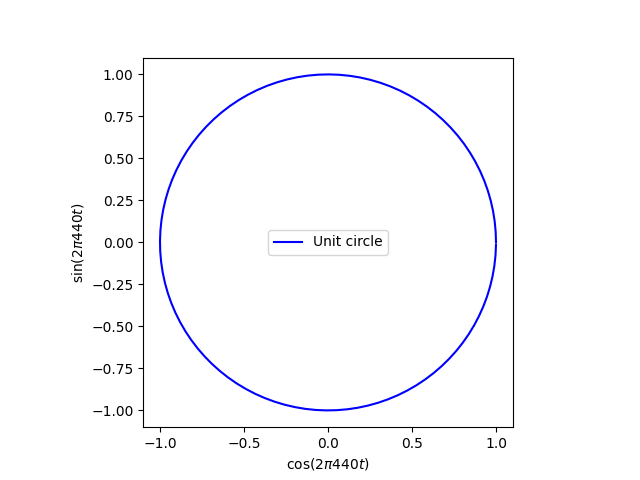
\includegraphics[width=\textwidth]{ch02/figures/circle_plot.png}
                  \caption{Output of Listing \ref{circle_plot}}
                \end{marginfigure}

          % Exercise 2d)
          \item The unit circle can be described by the equation $x^{2} + y^{2} = 1$, which is satisfied by $x = \cos(t)$ and $y = \sin(t)$.
        \end{enumerate}

  % Exercise 3
  \item Listing \ref{ipi} shows how to compute and print $e^{i\pi}+1$ in Python. The resulting output is \verb|1.2246467991473532e-16j|, which is not zero.
        The reason for this is due to floating point errors. The value is very close to 0, but not exactly 0.

        \lstinputlisting[language=Python, caption=Computing $e^{i\pi}+1$, label=ipi]{ch02/code/ex2_3.py}

  % Exercise 4
  \item The following is a solution for Exercise 4.

        \begin{enumerate}[a)]
          % Exercise 4a)
          \item Running the code generates the plot shown in the exercise.

          % Exercise 4b)
          \item Adding comments in Python can be done using \verb|#|, Listing \ref{comments_on_code} shows some comments.
                \lstinputlisting[language=Python, caption=Commented Python code, label=comments_on_code]{ch02/code/ex2_4.py}

          % Exercise 4c)
          \item One can specify the datatype of a NumPy array. The data types supported can be found in the documentation.
                These include: \verb|complex64|, \verb|complex128|, \verb|float32|, \verb|int32|, among others.
                Pros and cons with the \verb|complex64| and \verb|complex128| include: size and accuracy. The \verb|complex64|
                takes less memory, but is less accurate, while \verb|complex128| can store more accurate numbers, but takes more memory.

        \end{enumerate}

\end{enumerate}
